\newpage
\chapter{Theoretical Framework}
\label{chap1}
\textcolor{red}{ This chapter should contains all theory needed for SM:
\begin{itemize}
    \item Describe the elementary particles 
    \item Describe the fundamental interactions and their related fields
    \item Describe the EWSB and Higgs physics introduction
    \item Brief introduction to p-p collision and higgs production at LHC
    \item Discovery of Higgs boson at CERN 2012
    \item Higgs self coupling anomaly
    \item Describe Di-Higgs production as a direct process to measure higgs self coupling and probe of BSM effects
    \item Early Run 2 results and limits on \kl
    \item Introduction to EFT as an alternative interpretation of Full Run 2 results to probe physics at large scale 
\end{itemize}
}
\section{Introduction}
\label{chap1:intro}

\textcolor{red}{This section should include a brief history of particle physics and the SM. \\
}
How the world around us made? How does it work? These are questions asked a long-ago to understand the Universe. The first efforts to elucidate those questions referred to ancient Greek philosophers. Greeks gave much to the physics by developing the fundamental basis of modern principles as the conservation of matter, atomic theory. Democritus's model introduces Atom as small indivisible building blocks (particles) that matter consists off. At that time, atoms allowed to describe a variety of phenomena. Rutherford comes in 1909 with his experience says that atoms consist of mostly space with Electrons surrounding a dense central nucleus made up of Protons and Neutrons. At meantime, Newtonian laws of motion and atoms consist off a solid framework. Currently, the Standard Model (SM) is the most accurate model describing the universe composition. In the SM, there are two types of elementary particles: fundamental constituents of matter called "Fermions", and the quanta of fields called "Bosons" exchanged between when an interaction occurs between fermions. The SM has been successfully, so far, at predicting the results from the measurements performed in the past 50 years. The following sections provide more details about the standard model and its particles.
\section{Standard Model (SM) of particle physics}
\label{chap1:SM}
A possible goal of physicists is to reduce all natural phenomena to a set of fundamental laws and theories which, at least in principle, can quantitatively explain and predict experimental results. At the microscopic scale, all matter behaviour and phenomenology, including molecular, atomic, nuclear, and subnuclear physics, can be explained under three fundamental interactions: electromagnetic, weak and strong forces. At the macroscopic scale, the fourth force, the gravitational interaction, has an essential role, while it is negligible at the microscopic scale. All the three interactions are describes within a local relativistic Quantum Field Theory (QFT) based on the principal gauge invariance. This is called "The Standard Model". Within the SM matter consists of fermions and interactions are mediated by bosons. 

\subsection{Elementary Particles}
\label{chap1:SM:EP}
\textcolor{red}{
This should include a description of elementary particles, Fermions and  Bosons and their properties (mass, spin, charge, quantum number)
\\ }

In the SM, particles classified as either fermions or bosons depending on what statistics they obey. Fermions obey Fermi-Dirac statistics and respect the Pauli exclusion principle, i.e. two fermions in the same quantum state can not exist in the same place and time. Such particles have an intrinsic angular momentum, called spin J, half-integer. Bosons obey Bose-Einstein statistics, due to spin-statistics theorem, they have integer spin value. Through an interaction, a boson emitted by a matter particle and then absorbed by another particle. Fermions divided into two categories: Leptons and Quarks.
\subsubsection{Leptons}
Leptons (comes from the Greek word meaning "light") are grouped into three families or generations formed by three charged leptons: electron e, muons $\mu$ and tau $\tau$ with electric charge -e, with e being the elementary charge of $\sim 1.6 \ 10^{-19} $C, and their neutral complemented partners neutrinos : $\nu_{e}, \nu_{\mu}$ and $\nu_{\tau}$. Only electron and neutrinos (in SM) are stable. A quantum number called Leptonic number (L) is associated with each lepton. Electron, muon and tau have identical properties (a charge, spin) however tau is 3477 times heavier than an electron, the muon has 17 times the mass of an electron. The rest mass of an electron is $9.10938356 \ 10^{-31} Kg$. From 20 May 2019 kilogram not anymore part of the International System of Units for that masses will be expressed by the unit of energy (E) the electron-volt (eV) in this thesis. Mass is related to eV by the equation $E=mc^2$, c is the velocity of light in vacuum. In particle and high energy physics, c is fixed to one. Electron mass is $511 \ keV$.
\subsubsection{Quarks}
Quarks are electrically charger particles, with charge of $+\frac{2}{3}e$ for so-called up-type quarks and $-\frac{1}{3}e$ for the down-type quarks. There are six known quarks flavours, similarly to leptons, quarks are paired into three generations. The first generation consists of up (u) and down (d) quarks, the second has the charm (c) and strange (s) quarks, and top (t) and bottom (b) quarks for the third generation. Quarks can not exist in a free state (\textbf{More detail}). Table \ref{tab:fermions} shows a summary of leptons and quarks. \\
Each of the higher generations has particles with higher mass and tends to decay to the lower one, explains why the ordinary matter made off the first-generation particles. Each fermion has it is corresponding anti-particle.
\begin{table}[ht]
\centering
\begin{tabular}{c|c|c|c|}
\cline{2-4}
 &
  1st Generation &
  2nd Generation &
  3rd Generation \\ \hline
\multicolumn{1}{|c|}{Quarks} &
  \begin{tabular}[c]{@{}c@{}}u\\ 2.16 MeV\\ $+\frac{2}{3}$\end{tabular} &
  \begin{tabular}[c]{@{}c@{}}c\\ 1.27 GeV\\ $+\frac{2}{3}$\end{tabular} &
  \begin{tabular}[c]{@{}c@{}}t\\ 172.4 GeV\\ $+\frac{2}{3}$\end{tabular} \\ \cline{2-4} 
\multicolumn{1}{|c|}{} &
  \begin{tabular}[c]{@{}c@{}}d\\ 4.67 MeV\\ $-\frac{1}{3}$\end{tabular} &
  \begin{tabular}[c]{@{}c@{}}s\\ 93 MeV\\ $-\frac{1}{3}$\end{tabular} &
  \begin{tabular}[c]{@{}c@{}}b\\ 4.18 GeV\\ $-\frac{1}{3}$\end{tabular} \\ \hline
\multicolumn{1}{|c|}{Leptons} &
  \begin{tabular}[c]{@{}c@{}}e\\ 0.511 MeV\\ -1\end{tabular} &
  \begin{tabular}[c]{@{}c@{}}$\mu$\\ 105.7 MeV\\ -1\end{tabular} &
  \begin{tabular}[c]{@{}c@{}}$\tau$\\ 1.8 GeV\\ -1\end{tabular} \\ \cline{2-4} 
\multicolumn{1}{|c|}{} &
  \begin{tabular}[c]{@{}c@{}}$\nu_{e}$\\ 0\\ 0\end{tabular} &
  \begin{tabular}[c]{@{}c@{}}$\nu_{\mu}$\\ 0\\ 0\end{tabular} &
  \begin{tabular}[c]{@{}c@{}}$\nu_{\tau}$\\ 0\\ 0\end{tabular} \\ \hline
\end{tabular}
\caption{Generations of quarks and leptons with their masses and charges}\label{tab:fermions}
\end{table}
Standard Model of elementary particles assumes neutrinos to be mass-less particles, while some experiments demonstrate that neutrinos have a non-negligible mass $\sim eV$, which makes it an incomplete theory.
\subsubsection{Bosons}
As mentioned before, bosons are particles of integer angular momentum and obey to the Bose-Einstein statistics. They are the carriers of the gauge interactions between fermions. Photon ($\gamma$) is a boson known as a quantum of the electromagnetic field including electromagnetic radiation such as light. Photons are neutral and mass-less particles.  $W^{\pm}, Z^{0}$ are bosonic particles wish carriers the weak interaction. $Z^{0}$ boson is neutral while $W^{\pm}$ charged with a charge of $\pm$e. Contrary to photons, Weak bosons are massive. $W^{\pm}$ and $Z^{0}$ masses are predicted to be so large that it took many years to build powerful accelerators to produce them. $W^{\pm}$ and $Z^{0}$ bosons have been discovered at CERN in 1983 by the UA1 and UA2 collaborations, and their masses were found to be about 80 GeV and 91 GeV respectively. Gluons are the neutral quantum of the strong force known as the "glue" that links quarks to form hadrons. The mass of the gluons is known to be strictly zero. There are eights gluons. 
\subsection{Elementary Interactions}
\label{chap1:SM:EI}
\textcolor{red}{This should include a description of the 4 interaction and their properties.\\
The associated group for each of the SM interactions (U(1) SU(2) SU(3)) and the its Lagrangian.\\
How SM combines the 3 groups in one fundamental theory which describe particle physics.\\
Brief summary of boson vs interactions
} \\
There are three conventionally taken fundamental forces (other than gravitation) electromagnetic, weak and strong. The interactions relate to matter (fermions) by the transmission of a boson. The SM content and interactions can be expressed more formally through the concepts of symmetries and gauge invariance. Each interaction is described through a gauge group. The generators of the group correspond to the gauge bosons that are mediators of the fundamental force and responsible for the interactions. As mentioned above, Electromagnetic interaction mediated by photons. Weak forces used $W^{\pm}$ and $Z^{0}$ as mediators while the Gluons are mediators for the strong interaction.
\subsubsection{Electromagnetic interaction}
Electromagnetic interaction describes the dynamics of charged fermions. It is described by the Quantum Electrodynamics (QED). Each quantum field theory is represented by a Lagrangian density, the QED Lagrangian representing the behaviour of a freely propagating fermion field $\psi (x,t)$ can be written as : 
\begin{equation}
    \mathcal{L} = \bar{\psi}i\gamma^\mu\partial_\mu\psi - m\psi\bar{\psi},
\end{equation}
where m is the mass of the particle. The Einstein convention is used here, with the indices $\mu= 0,1,2,3$ representing the space-time components x and t. \\ 
To be a valid gauge theory the QED lagrangian should be invariant under a U(1) (electromagnetic force group) local gauge transformation of the field : $\psi\rightarrow e^{i\alpha(x)}\psi$. This condition leads to additional terms to be added to the lagrangian and new gauge field $A_{\mu}$ that represents the photon:
\begin{equation}
    \mathcal{L}_{QED} = \bar{\psi}i\gamma^\mu\partial_\mu\psi - m\psi\bar{\psi} + q\psi\gamma^{\mu}\psi A_{\mu} - \frac{1}{4}F^{\mu\nu}F_{\mu\nu},
\end{equation}
where $F^{\mu\nu} = - F^{\mu\nu} = \partial^{\nu}A^{\mu} - \partial^{\mu}A^{\nu}$ is the field-strength tensor for the electromagnetic force, as described by Maxwell equations, describes the kinetic propagation of the field. Note that U(1) is an Abelian group, this means that photons can not self-interact and the EM tensor does not have the photon self-interaction term included. The term $q\psi\gamma^{\mu}\psi A_{\mu}$ reflects the interaction between a fermion and the electromagnetic force (photon) with strength q (q=-e) the electromagnetic interaction charge (electric charge). The mass term of the photon is not added to the lagrangian since it spoils the gauge invariance. This is in agreement with the observation that the photon is mass-less. U(1) has one generator corresponds to the photon mediator.
\subsubsection{Electro-Weak interaction}
Electroweak consists of an unification of the electromagnetic and weak interactions. It is described by the combined gauge symmetry $SU(2)_{T}\times U(1)_{Y}$, where the $U(1)_{Y}$ symmetry mimics that of QED with the weak hypercharge Y. The $SU(2)$ represents the weak interaction with its generator vector T called weak isospin. The Lagrangian of the theory can be written as : 
\begin{equation}
    \mathcal{L}_{EW} = \bar{\psi}i\gamma^\mu\partial_\mu\psi -eY\bar{\psi}\gamma^{\mu}B_{\mu}\psi-g_{W}\bar{\psi}\gamma^{\mu}\textbf{T.W$_\mu$}\psi
    -\frac{1}{4}F^{\mu\nu}F_{\mu\nu} - \frac{1}{4}W^{i\mu\nu}W^i_{\mu\nu},
\end{equation}
where $g_{W}$ is the weak coupling to the fermionic fields. The first two terms are similar to $\mathcal{L}_{QED}$. However, the term representing the coupling of fermions to photons is replaced by more general terms, and the $W_{\mu}$ field and the hyper-photon $B_{\mu}$ field are introduced. The two charged vector bosons $W^\pm$ appear as linear combinations of the $W_{\mu}$ field components, $W^{\pm}_{\mu} = \frac{1}{\sqrt{2}}(W^1_{\mu}\mp W^2_{\mu})$. The photon is now created through the mixing of the $W_{\mu}$ and $B_{\mu}$ fields, as :
\begin{equation}
    A_{\mu} = B_{\mu}cos\theta_{W} + W^3_{\mu}sin\theta_{W},
\end{equation}
where $\theta_{W}$ is the weak mixing angle, and the $Z_{\mu}$ field, corresponding to the Z boson, is generated similarly as : 
\begin{equation}
     Z_{\mu} = -B_{\mu}sin\theta_{W} + W^3_{\mu}cos\theta_{W}.
\end{equation}
The field strength tensor for the weak gauge fields $W^i$ is defined as:
\begin{equation}
    W^{i}_{\mu\nu} = \partial_{\mu}W^i_{\nu} - \partial_{\nu}W^i_{\mu} - g_{W}\epsilon_{ijk}W^i_{\mu}W^i_{\nu},
    \label{eq:W}
\end{equation}
The non-Abelian nature of SU(2) generates the third term in Eq.(\ref{eq:W}), wish gives rise to the weak boson self-interactions. \\
The electric charge q is related to Y and T by through the Gell-Mann-Nishijima relation:
\begin{equation}
    q = T_3 + \frac{Y}{2},
\end{equation}
where $T_3$ is the third component of the isospin $T$.
Fermions are decomposed into left-handed and right-handed chirality types. The chirality is defined for mass-less particles as the same as hilicity and refers to the relation between the spin and momentum direction. While for massive particles chirality is trickier to define. Note that the electroweak force interacts only with left-handed particles and the right-handed anti-particles, violating the parity. The chirality distinct between left-handed doublets, and the right-handed singlets:
\begin{equation}
    (\nu_i \ i)^T_L, i_R \ with i = e, \mu \ or \ \tau,
\end{equation}
and, 
\begin{equation}
    (u \ d)^T_L, \ (c \ s)^T_L, \ (t \ b)^T_L, \ u_R, \ d_R ... \ . 
\end{equation}

\subsubsection{Strong interaction}
Additionally to QED, the strong interaction is described by Quantum Chromo-Dynamics (QCD), which is a local gauge symmetry under $SU(3)_C$. SU(3) has eight generators correspond to the eight gluons mediators of the strong force. The expression for the locally gauge invariant Lagrangian of the QCD, which describes interactions of quarks of mass m and quark-field spinors $\psi$ via a mass-less gluons is:
\begin{equation}
    \mathcal{L}_{QCD} = \sum_{flavours} \bar{\psi}_a(i\gamma^\mu\partial_\mu\delta_{ab}-g_{s}\gamma^\mu t^C_{ab}G^C_\mu - m\delta_{ab})\psi_b - \frac{1}{4}F^A_{\alpha\beta}F^{A\alpha\beta},
\end{equation}
where a = 1,2,3 is the color index. The $G^{C}_\mu$ are the gluon fields with C= 1,2,..,8 that transform under the adjoint representation of the SU(3) group.  The $t^C_{ab}$ are the generators of the SU(3) group, the quantity $g_{s}$ corresponds to strong coupling constant that determines the strength of interactions between coloured particles (quarks and gluons). The strong field tensor is defined as :
\begin{equation}
    F^A_{\alpha\beta} = \partial_\mu G^A_\nu - \partial_\nu G^A_\mu - g_sf^{ABC}G^B_\mu G^C_\nu,
 \end{equation}
where $f^{ABC}$ are the structure constants of the SU(3) group. In contrast to QED, the field tensor of the QCD includes the gluon triplet and quartic self-interactions. Only particles carrying colour charge (i.e.quarks) couple to these gluons. Colour charge is conserved in each interaction. Since the SU(3) group is non-Abelian, the gluons themselves must also carry (anti-)colour charge and thus interact with each other. \\

Finally, the standard model Lagrangian density could be summarized as : 
\begin{equation}
    \mathcal{L}_{SM} \sim \mathcal{L}_{EW} + \mathcal{L}_{QCD}.
\end{equation}
Note that, in the $\mathcal{L}_{EW}$ no mass term is introduced for the two newly appearing bosons, while experimental observations were found that indicate they were massive. Additionally, the fermion mass term that appeared in $\mathcal{L}_{QED}$ is now absent in $\mathcal{L}_{EW}$, requiring the introduction of an additional mechanism to explain the origin of their mass. This is handled through the process of Electroweak Symmetry Breaking (EWSB), and the introduction of the Higgs mechanism to generate mass.

\section{Electroweak Symmetry Breaking (EWSB)}
\label{chap1:EWSB}
\textcolor{red}{This section will ask the question mass of particles and introduce the EWSB to answer.\\
Introduce the Higgs boson and its proprieties.\\
}
The gauge bosons mass terms are not introduced as would break gauge invariance. Brout-Englert-Higgs (BEH) mechanism introduces a spontaneous symmetry breaking ad-hoc in the SM to preserve the local gauge invariance. In the minimal model of EWSB, mass of particle can be generated by introducing the Higgs field represented by a weak iso-spin doublet of one charged and one neutral complex scalar (J=0) field complex scalar :
\begin{equation}
    \phi(x)=\frac{1}{\sqrt{2}}\left(\begin{array}{c}
\phi_{+} \\
\phi_{0}
\end{array}\right).
\end{equation}
Higgs lagrangian is added to the SM lagrangian as :
\begin{equation}
    \mathcal{L}_{\mathrm{Higgs}}=\left(D^{\mu} \phi\right)^{\dagger}\left(D_{\mu} \phi\right)-V(\phi),
\end{equation}
where $D^\mu$ is the covariant derivative $D^\mu =\left(\partial_{\mu}+i g T^{i} W_{\mu}^{i}+i \frac{1}{2} g^{\prime} B_{\mu}\right)$. The kinetic and the interaction of the Higgs field with weak gauge bosons is described by the term $D^\mu\phi$. $V(\phi)$ is the Higgs potential:
\begin{equation}
    V(\phi)=\mu^{2} \phi^{+} \phi+\lambda\left(\phi^{+} \phi\right)^{2},
\end{equation}
the first term can be associated to the mass of the field and the second represents the quadratic self-interaction of the scalar field. The parameter $\lambda$ has to be to be positive to obtain a potential with finite minima, while $\mu$ can be chosen freely. For $\mu^{2} > 0$, the potential has a single ground state at zero with all fields being zero ($\phi_0 = 0$). Hence the vacuum expectation value of the Higgs field would be zero and the symmetry is preserved. However, for $\mu^{2} < 0$ the potential has an infinite set of minima $v$ given by :
\begin{equation}
    \phi_{0}=<\phi^{+} \phi>=\frac{v^{2}}{2}=-\frac{\mu^{2}}{2 \lambda},
\end{equation}
$v\neq0$ being the vacuum expectation value (vev) which is shown in \ref{fig:chap1:Higggs_potential}.
\begin{figure}[ht]
    \centering
    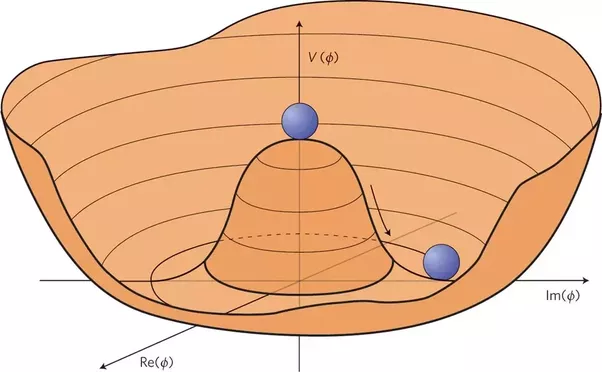
\includegraphics[width=0.5\textwidth]{Ch1/Img/Higgs_potential.png}
    \caption{Shape of the Higgs potential for $\mu^{2} < 0$ this potential has an infinite amount of minima.}
    \label{fig:chap1:Higggs_potential}
\end{figure}
\\
The choice of the physical vacuum state spontaneously breaks the Lagrangian symmetry. An expansion of $\phi_0$ around its vacuum state $v$ introduces a massive scalar and three mass-less Gladstone bosons. However, the Goldstone bosons appear to be not physical and can be eliminated using the gauge Unitary, enforcing the Higgs doublet to be real:
\begin{equation}
    \phi(x)=\frac{1}{\sqrt{2}}\left(\begin{array}{c}
0 \\
v+h(x)
\end{array}\right),
\end{equation}
where $h(x)$ is physical field linked to the Higgs boson. The form of Higgs potential becomes: \begin{equation}
    V(\phi)=-\frac{1}{2} m_{H}^{2} h^{2}(x)+\lambda_{H H H} h^{3}(x)+\lambda_{H H H H} h^{4}(x),
\end{equation}
where $m_{H}^{2}=2 \lambda^{2}=2 \lambda v^{2}$ is the square of Higgs mass, $\lambda_{HHH}$ is the coupling in a vertex with tree Higgs and $\lambda_{HHHH}$ for the case of four Higgs.
Accordingly, the terms giving the mass to the gauge bosons can be identified:
\begin{equation}
m_{W} = \frac{1}{2}gv 
\end{equation}
\begin{equation}
m_{A} = 0    
\end{equation}
\begin{equation}
m_{Z} = \frac{m_{W}}{\cos\theta_{W}}.
\end{equation}
The Higgs mechanism associates the degrees of freedom of hypothetical scalar (Goldstone) bosons with the longitudinal components of gauge bosons and consequently become massive. The coupling of the Higgs boson to the gauge bosons appears to be proportional to the gauge boson masses. The mass of the fermions not explained in the same way. However, the fermions acquire masses through the corresponding Yukawa couplings.  Weak bosons masses are predicted in the SM, while  Higgs boson mass is unknown and could have any value. Higgs mass needs to be measured, and the Higgs boson discovery is necessary to confirm the EWSB.
\section{Higgs Boson Discovery}
\label{chap1:H2012}
\textcolor{red}{This should contains the story of Higgs boson discovery by ATLAS and CMS in 2012. \\}
The Large Electron Positron (LEP) collider approved by the CERN Council in 1981 and commissioned eight years later, provides a detailed study of the electroweak interaction for 11 years of research. Results from LEP are used to perform stringent tests of the SM by comparing the precise results with theory predictions. LEP allows us to measure the masses of heavy fundamental particles, such as the top quark and the W boson, which are then compared to the predictions. This checks the correctness of the SM predictions. Constrain the Higgs mass is a particular interest, because this fundamental ingredient of SM has not been observed and needed to complete the SM picture. At the beginning of the LEP program no solid limit existed on the mass of the Higgs boson. The searches for the SM Higgs boson carried out by the four LEP experiments extended the sensitive range well beyond that anticipated at the beginning of the LEP program. This is due to the higher energy achieved and to more sophisticated detectors and analysis techniques. However, circular accelerators with electrons is limited by synchrotron radiation due to the small electron mass. Since muon acceleration is not possible at the current stage due to the short life time of muons, proton collisions represent a good way to achieve high-energy collisions needed for Higgs discovery. LEP was closed down on 2 November 2000 to make way for the construction of the Large Hadron Collider (LHC) in the same tunnel. LHC provides mainly proton-proton collisions at a centre-of-mass energy of $\sqrt(s)$ up to 13. LHC is detailed in a dedicated Chapter \ref{LHC&ATLAS}. 
\subsection{p-p collisions}
\label{chap1:H2012:PP}
\textcolor{red}{The protons protons collision and the Higgs boson cross section at 8 TeV and 13 TeV. \\}
Protons are fermions known to be made up of two up and one down quarks ($uud$) called valence quarks. They interact between each other through the strong force via gluon exchange. Due to nature of QCD (non-abelian) gluons can fluctuate into quark anti-quark pairs forming the so-called sea quarks. Effectively, a proton is therefore a bound state of quarks and gluons called partons each carries a fraction $x$ of the total proton momentum. At LHC process are produced by colliding mainly protons beams, similarly Higgs boson processes are in p-p collision.
\begin{equation}
    p_1 + p_2 \rightarrow h.
\end{equation}
The probability for a process to occur is expressed in terms of its cross section, and the dynamics of its products is determined by the dynamics of partons involved in the collision. The hard scattering cross section for such process is given by :
\begin{equation}
    d \sigma^{p_{1} p_{2} \rightarrow h}=\int_{0}^{1} d x_{1} \int_{0}^{1} d x_{2} \sum_{a, b} f_{a / p_{1}}\left(x_{1}, \mu_{F}^{2}\right) f_{b / p_{2}}\left(x_{2}, \mu_{F}^{2}\right) d \hat{\sigma}^{a b \rightarrow h}\left(x_1, x_2, \mu_{F}^{2}\right), 
\end{equation}
where $a$, $b$ are the partons involved in the process and $f_{n/p_i}(x_i)$ is the parton distribution function (PDF), which is the probability to find a parton of type $n$ inside proton $p_i$ with a longitudinal momentum fraction $x_i$ at energy scale $Q$. $\sigma^{a b \rightarrow h}$ is the parton cross section of the process. \\
In general, the x dependence at a given $Q^2$ cannot be calculated analytically but rather are extracted from global fits to data from many experiments. There are different PDF sets which use different fitting methods and experimental data. Figure \ref{fig:chap1:H2012:PDF} shows two examples of CT14 PDFs at given $Q^2$. 
\begin{figure}[ht]
    \centering
    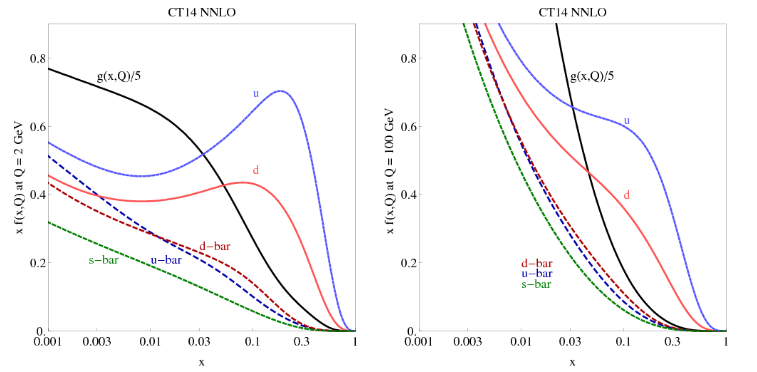
\includegraphics[width=\textwidth]{Ch1/Img/PDFs.png}
    \caption{The CT14 PDFs at Q=2 GeV (left) and Q = 100 GeV (right) for different partons. These PDFsare computed at next-to-next-to-leading order.}
    \label{fig:chap1:H2012:PDF}
\end{figure}
\\
The production of the Higgs boson at the LHC occurs in different modes. Their cross sections depend on the coupling of the Higgs boson to specific particles, but also essentially on the PDFs described above.
\subsection{Higgs boson production}
\label{chap1:EWSB:HP}
\textcolor{red}{Higgs boson production modes ggF VBF VH and qqH. \\}
The main process contributing to the Higgs boson production at LHC are represented by their leading Feynman diagrams in Figure \ref{fig:chap1:EWSB:HP}. The most important Higgs production mode occurs via fusion of gluons (ggF). 
\begin{figure}[ht]
    \centering
    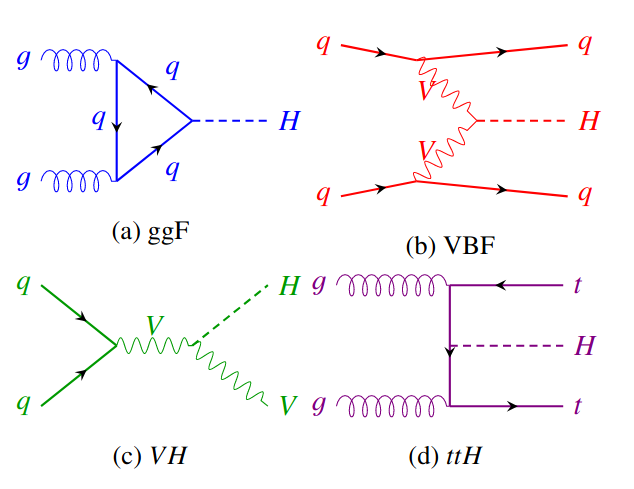
\includegraphics[width=0.5\textwidth]{Ch1/Img/Higgs_prod_modes.png}
    \caption{Feynman diagrams for the main production modes of Higgs boson.}
    \label{fig:chap1:EWSB:HP}
\end{figure}
In order of decreasing cross section, the Higgs boson production modes are:
\begin{itemize}
	\item gluons-gluons fusion (ggF) : the main Higgs boson production at LHC over the whole mass spectrum. The process involves the fusion of two incoming gluons that give rise to the Higgs boson through a heavy quark loop, whose main contribution comes from the top quark, as shown in Figure \ref{fig:chap1:EWSB:HP} (a).  
	\item Vector Boson Fusion (VBF) : each of the two interacting quarks emit a W or Z boson which, in turn, interact to produce the Higgs boson, as shown in figure \ref{fig:chap1:EWSB:HP} (b). Quarks deriving from the incoming partons after the emission of vector bosons proceed in the forward direction and represent the peculiar signature of this production mode, two high energy forward jets separated by a large pseudo-rapidity gap, a $\Delta\eta$ region with reduced particle density. This process has a cross section which is one order of magnitude lower than ggF for a large range of Higgs boson mass ($m_H$) values and it becomes comparable to ggF only for masses of the order of 1 TeV as shown in Figure \ref{fig:chap1:EWSB:HXSEC} (b).
	\item Vector boson associated production (VH) : also known as Higgs strahlung, this process is characterized by the emission of a Higgs boson from a $W^{\pm}$ or $Z$ boson produced by two incoming quarks, as shown in figure \ref{fig:chap1:EWSB:HP} (c). The VH cross section is several orders of magnitude lower than the ggF and VBF cross sections for $m_H$ larger than about 300 GeV, while the VH and VBF cross sections are comparable around $m_H = 125$ GeV as shown Figure \ref{fig:chap1:EWSB:HXSEC} (b).
	\item Top quark associated production ($t\bar{t}H$) : a pair of top quarks, originated from the splitting of two incoming gluons, interacts to give rise to a Higgs boson, as shown in figure \ref{fig:chap1:EWSB:HP} (d). the production in association with a pair of top quarks allows a direct measurement of the Higgs boson coupling to the top quark. Another production mechanism analogous to the $t\bar{t}H$ process and with a similar cross section is the b-quark associated production.
\end{itemize}
The SM Higgs boson production cross section for the various production modes depends on the Higgs boson mass and on the center-of-mass energy, as shown in Figure \ref{fig:chap1:EWSB:HXSEC}.  
\begin{figure}[ht]
    \centering
    \subfloat[][]{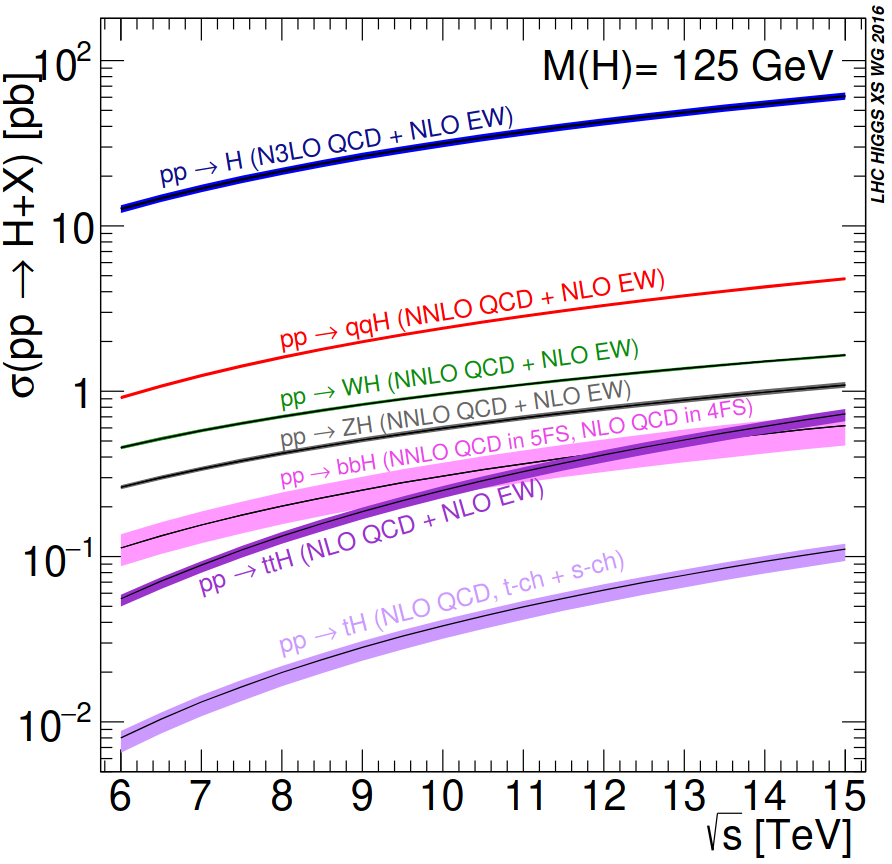
\includegraphics[width=.51\textwidth]{Ch1/Img/Higgs_Xsec_s.png}}
    \subfloat[][]{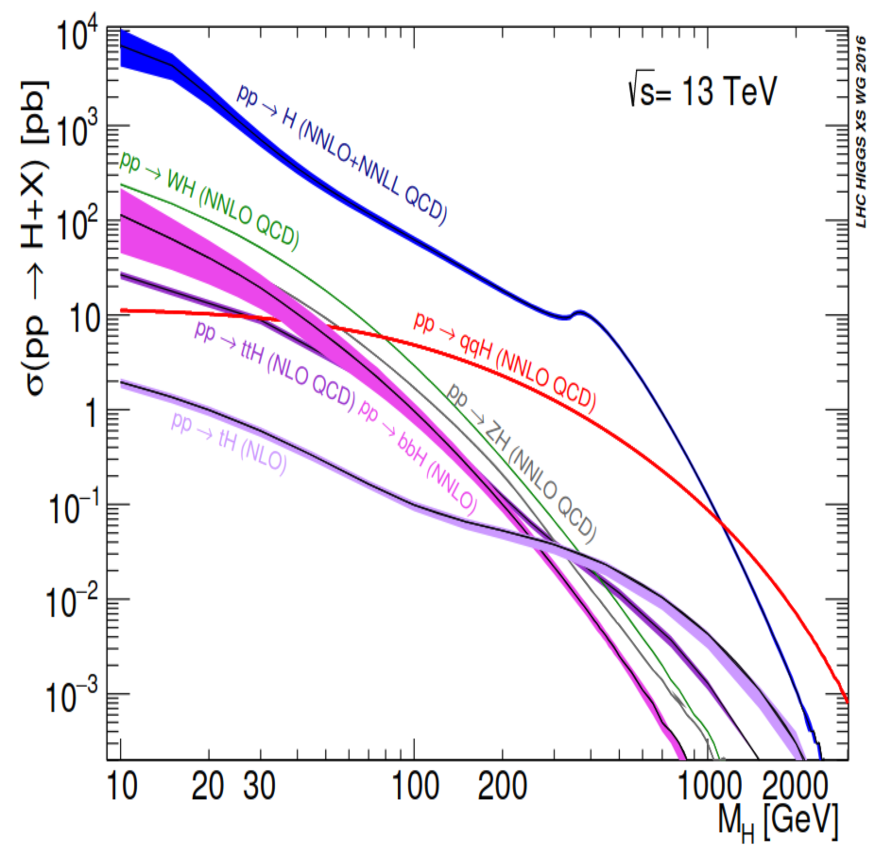
\includegraphics[width=.52\textwidth]{Ch1/Img/Higgs_Xsec_mass.png}}
    \caption{Cross sections for different Higgs boson production modes at a proton-proton collider with a centre-of-mass energy of 6-15 TeV (a). A Higgs mass of 125 GeV is assumed in this plot. Additionally, cross sections as a function of Higgs mass are shown (b).}
    \label{fig:chap1:EWSB:HXSEC}
\end{figure}
Higgs boson is a unstable particle as shown in Figure \ref{fig:chap1:EWSB:D}, note that the probability to decay within a given time "decay width" $\Gamma$ is linked to the lifetime $\tau$ by $ \Gamma\tau = \hbar$ where $\hbar$ is the reduced Planck constant. In order to identify Higgs and its production modes, it is reconstructed from its products for a chosen decay channel. 
\begin{figure}[ht]
    \centering
    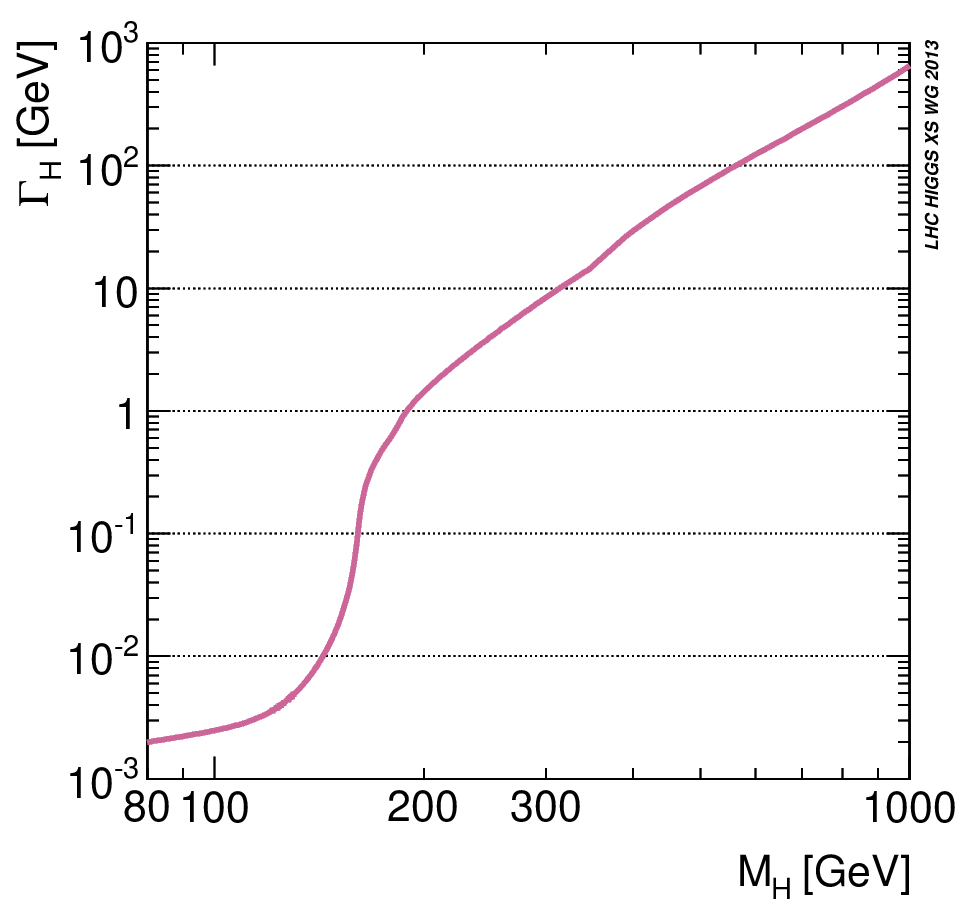
\includegraphics[width=0.5\textwidth]{Ch1/Img/Higgs_decay.png}
    \caption{Higgs boson total decay width as a function of Higgs mass.}
    \label{fig:chap1:EWSB:D}
\end{figure}

\subsection{Higgs boson decay channels}
\label{chap1:EWSB:HD}
\textcolor{red}{Higgs boson decay modes and their rates. \\}
The possible SM Higgs boson decay modes are very depend on the Higgs boson mass as shown in figure \ref{fig:chap1:EWSB:BR} for a Higgs boson mass range of 80 to 200 GeV. If the Higgs boson were heavy enough to decay into two real vector bosons, the modes $H\rightarrow WW^*$ and $ H\rightarrow ZZ^*$ would have dominated the decay with small contribution from Higgs to di-top quarks. At very low masses of the Higgs boson, decays into vector boson or $t\bar{t}$ would have played almost no role and the dominant decay mode would have been the experimental challenging decay mode $H\rightarrow b\bar{b}$.
\begin{figure}[h!]
    \centering
    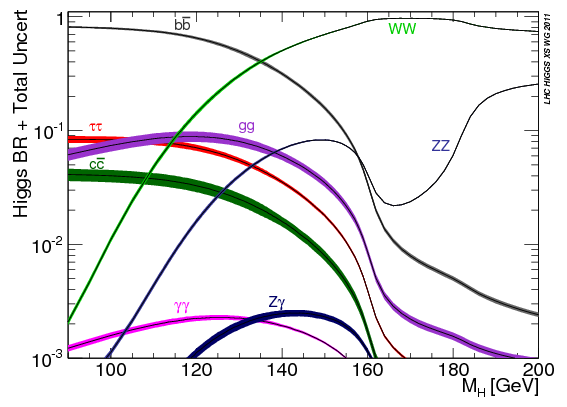
\includegraphics[width=0.5\textwidth]{Ch1/Img/Higgs_Br.png}
    \caption{Higgs boson branching ratio of the possible Higgs decay channels as a function of the Higgs mass.}
    \label{fig:chap1:EWSB:BR}
\end{figure}
Since photons are mass-less particles, the direct coupling of the Higgs boson to photons is zero in the SM. However, the Higgs boson can decay into a pair of photons via loop processes. The main Feynman diagrams of this decay are shown in Figure \ref{fig:chap1:EWSB:Hgg}. 
At a Higgs boson mass of 125 GeV, the dominant decay of the Higgs boson is $H \rightarrow b\bar{b}$ with a branching ratio of roughly 58\%. At the same mass $H\rightarrow\gamma\gamma$ branching ratio is around 0.23\%.
\begin{figure}[ht]
    \centering
    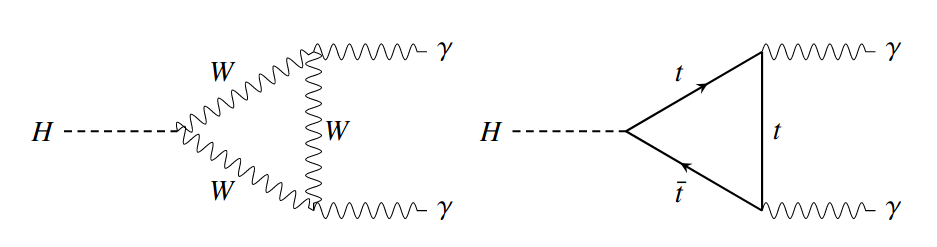
\includegraphics[width=0.5\textwidth]{Ch1/Img/H_to_gammagamma.png}
    \caption{Feynman diagrams of the $H\rightarrow\gamma\gamma$ decay. Other particles can also propagate in the loop.}
    \label{fig:chap1:EWSB:Hgg}
\end{figure}

\subsection{Higgs measurements}
\label{chap1:H2012:HM}
\textcolor{red}{The discovery of Higgs boson in 2012 by ATLAS and CMS and first measurements of its mass.
Recap of Higgs boson proprieties. and Introduction to self couplings no yet measured. \\
}
ATLAS and CMS collaborations, the two larges experiments of the LHC, announced on 4 July 2012 the identification with $99.99997\%$ ($5\sigma$) of a new boson within a mass range of $125-127 GeV$. The new boson matches the Standard Model Higgs boson proprieties. Later, was confirmed that the new particle, without doubt, corresponds to the Higgs boson. Higgs boson predicted in 1964, but the world had to wait until 2012 before its discovery by physicists at CERN. The Evidence of the new boson was present in the three bosonic decay modes $H\rightarrow ZZ^* \rightarrow 4l, H\rightarrow\gamma\gamma$ and $H\rightarrow WW^*\rightarrow l\nu l\nu$. The branching ratio of Higgs in the di-photon decay channel is small. Despite the comparably low branching fraction of this decay mode, their construction of two photons has a clean signature in the detector and allows a good energy resolution. This signal can therefore well be separated from the dominating continuum di-photon background from QCD jets, which has a smooth and well parametrisable shape. Which makes the expected Higgs boson signal significance in this decay mode is one of the highest among all the decay modes in the mass range $110 < m_{H} < 150 GeV$. Events in data collected in 2010 and 2011 with centre-of-mass energy $\sqrt{s}=7 TeV$ and $8 TeV$ respectively containing di-photons are combined to make the evidence of Higgs boson. Figure \ref{fig:chap1:H2012:Hyy} shows the weighted distribution of the invariant mass of photon pairs measured by ATLAS experiments. The distributions are obtained by summing the invariant mass distributions of all of the selected events, with each event being weighted by $S/B$ where S and B and the number of signal and background events, respectively. Figure \ref{fig:chap1:H2012:Hyy} demonstrates a statistically significant excess of events near 125 GeV. \\
\begin{figure}[h!]
    \centering
    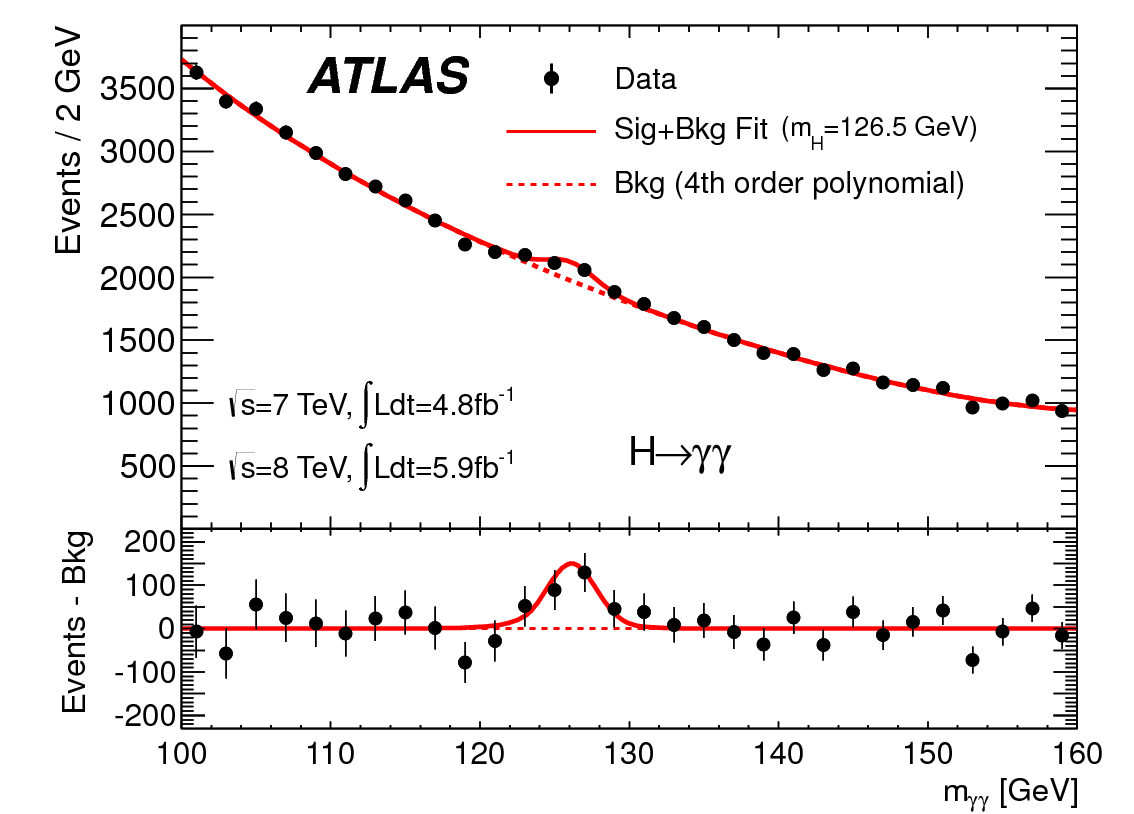
\includegraphics[width=0.5\textwidth]{Ch1/Img/Hmyy.png}
    \caption{Weighted distributions of the invariant mass of di-photon.}
    \label{fig:chap1:H2012:Hyy}
\end{figure}
Measurement of the three channels are combined to confirm the observation of the new particle. The observed local significance reaches $6\sigma$ (the observed signal is $\sim10^{-9}$ to be a background fluctuation) around 125 GeV making the first observation of Higgs boson, Figure \ref{fig:chap1:H2012:P0}.  
\begin{figure}[H]
    \centering
    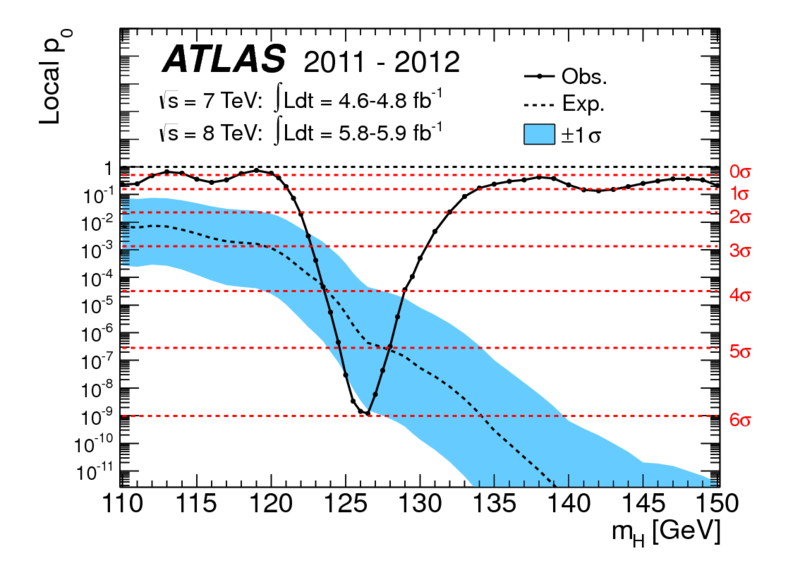
\includegraphics[width=0.5\textwidth]{Ch1/Img/Hp0.png}
    \caption{The observed local p-value as a function of $m_H$ (solid line) and the expectation with its $\pm1\sigma$ band assuming the presence of a Standard Model Higgs boson at that mass (dashed line) from the combination of the $ZZ^*$, $\gamma\gamma$ and $WW^*$ channels by the ATLAS experiment. The horizontal dashed lines indicate the p-values corresponding to significances of 1 to 6$\sigma$}
    \label{fig:chap1:H2012:P0}
\end{figure}
The latest measurement of Higgs boson yields to a  mass of $m_{H}=124.97\pm0.24 $ GeV. \\
Finally, by the observation of Higgs boson the last piece of the standard model of elementary particles is founded. SM particles are summarized in Figure \ref{fig:chap1:H2012:SM}.
\begin{figure}[ht]
    \centering
    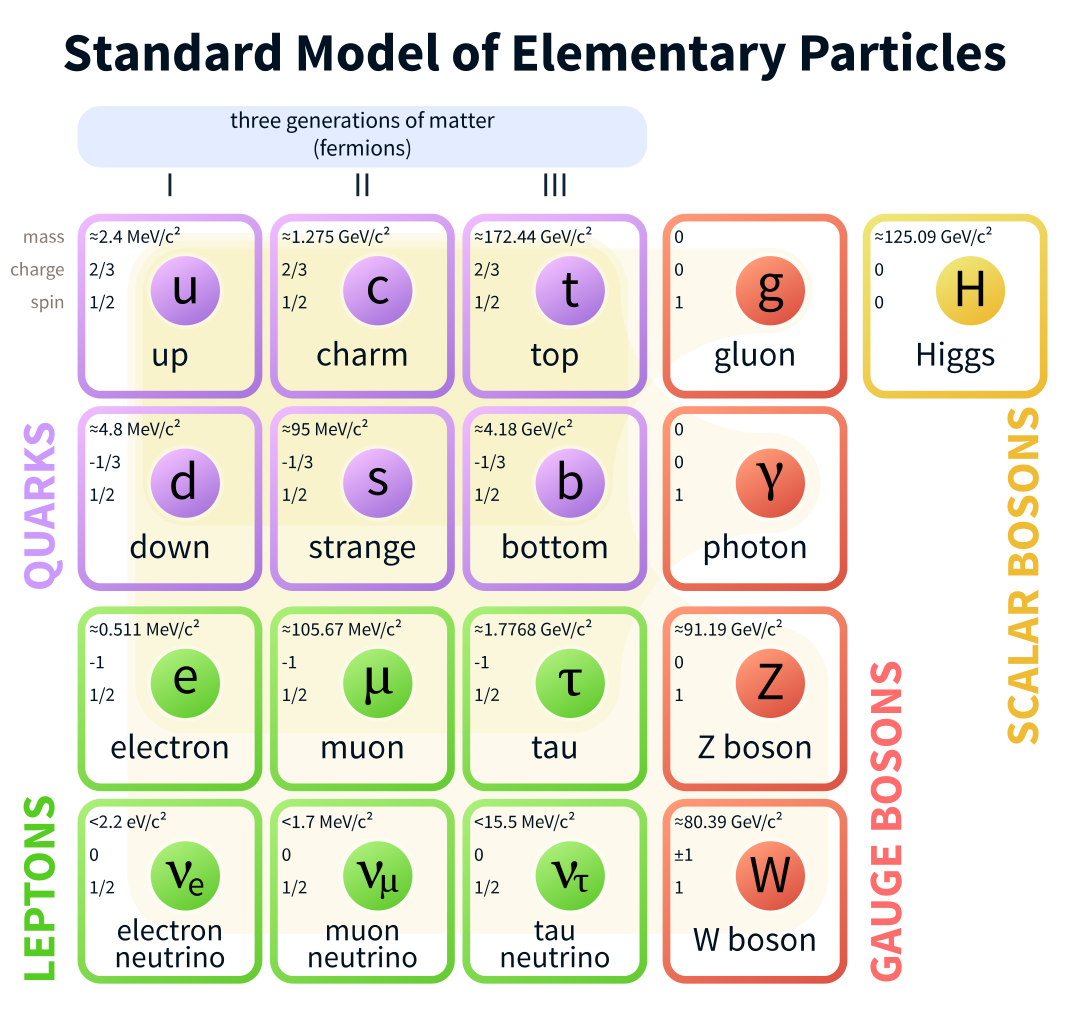
\includegraphics[width=0.5\textwidth]{Ch1/Img/SM_particles.png}
    \caption{The particle content of the Standard Model (SM).}
    \label{fig:chap1:H2012:SM}
\end{figure}
Understating the proprieties and couplings of the last piece of SM is a priority of both ATLAS and CMS. Higgs self-couplings $\lambda_{HHH}$ is vital, providing a direct probe on the EWSB and is a precision test of the electroweak theory. A direct probe of the trilinear coupling is possible through studying Higgs pair production where two Higgs boson are produced in the same event, making di-Higgs analyses particularly interesting and the main subject of the thesis.

\section{Double Higgs boson}
\label{chap1:HH}
\textcolor{red}{This should contain the theory of HH and how it allows to measure the higgs self couplings.
\\
}
Double Higgs production (HH) presents the alone direct measurement of the Higgs self-coupling.  Measuring HH is necessary to confirm the SM. In particular, the measurement of the Higgs boson self-coupling $\lambda$ (also referred to as the Higgs boson tri-linear coupling $\lambda_{HHH}$) is of great importance as expected to yield a deeper understanding of particle physics and cosmology. This measurement makes it possible to experimentally reconstruct the Higgs potential and check whether the Higgs boson discovered in 2012 at CERN is the one predicted by the Brout-Englert-Higgs mechanism. The di-Higgs production rate gives a handle to more accurately measure the Higgs potential. The main goal of this thesis is the search of Higgs boson pair production.
\subsection{Di-Higgs production and decays} 
\label{chap1:HH:HPD}
\textcolor{red}{This should contain the production modes and decays of HH. and the \HHyybb channel.
\\
}
As the SM provides the trilinear coupling of the Higgs boson, all SM Higgs boson production mode are known for di-Higgs production. Similarly to single Higgs boson, HH production is dominated by gluon-gluon fusion (ggF) through the destructive interference of two LO Feynman diagrams, shown in Figure \ref{fig:chap1:HH:HPD:FY}, involving top-quark loops and the triple Higgs self-coupling. In the box diagram, the top-quark Yukawa coupling $\lambda_t$ is present in two vertices so the contribution of this diagram to the amplitude is proportional to $\lambda_t^2$, while in the triangle diagram there is $\lambda_t$ in one vertex and the triple Higgs self-coupling $\lambda_{HHH}$ in the other vertex and the contribution of this diagram is proportional to $\lambda_t\cdot\lambda_{HHH}$. The amplitude of the process can be written as :
\begin{equation}
    A(\lambda_t, \lambda_{HHH}) \equiv \lambda_t^2\cdot\square + \lambda_t\cdot\lambda_{HHH}\bigtriangleup,
\end{equation}
where $\square$ represents the contribution of the box diagram and $\bigtriangleup$ the one of the triangle diagram. 
\begin{figure}[H]
    \centering
    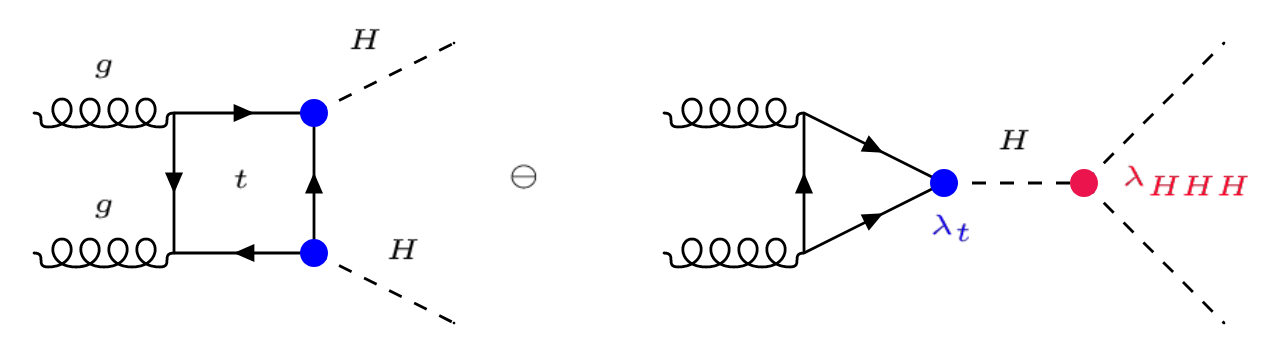
\includegraphics[width=0.8\textwidth]{Ch1/Img/HH_feyn.png}
    \caption{Leading Order (LO) Feynman diagrams contributing to ggF Higgs boson pair production through a top-quark loop (box) and through the triple self-coupling of the Higgs boson (triangle).}
    \label{fig:chap1:HH:HPD:FY}
\end{figure}
The SM cross section for Higgs boson pair production via ggF at $\sqrt{s}=13$ TeV, calculated at Next-to-Next-to-Leading Order (NNLO), is:
\begin{equation}
    \sigma_{HH}^{NNLO} = 33.53_{-6.0\%}^{+4.3\%} \ fb,
    \label{eq:chap1:HH:XSEC:NNL0}
\end{equation}
three orders of magnitude smaller than the single Higgs production cross section. This accounts for more than 90\% of the total Higgs boson pair production cross section. VBF mode also contribute to the di-Higgs production with a very low cross section (two orders of magnitude smaller). Therefore only the $ggF$ production mode is considered in this thesis. Figure \ref{fig:chap1:HH:HPD:FYS} shows the other production modes contributing to Higgs pair production. \\
Figure \ref{fig:chap1:HH:HPD:DCY} presents the matrix of the decay channels of Higgs boson pair resulting from all possible combination of decays of the two Higgs bosons. The dominants channels are $HH\rightarrow b\bar{b}b\bar{b}$, $HH\rightarrow b\bar{b}\tau\tau$ and $HH\rightarrow b\bar{b}WW^*$. 
\begin{figure}[H]
    \centering
    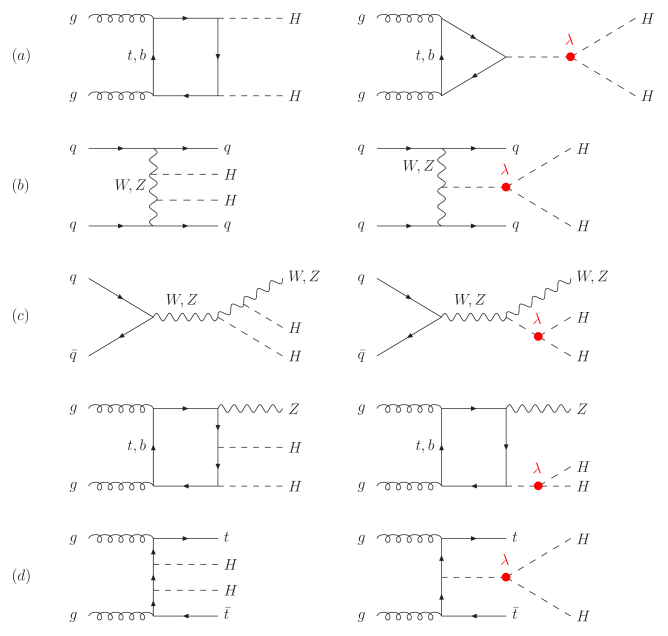
\includegraphics[width=0.65\textwidth]{Ch1/Img/HH_feyns.png}
    \caption{HH production modes, in decreasing order of cross section. $\lambda$ referees to Higgs tri-linear coupling: (a) ggF mode, (b) VBF mode, (c) Vector boson association (VH) and (d) top associated production.}
    \label{fig:chap1:HH:HPD:FYS}
\end{figure}
\begin{figure}[H]
    \centering
    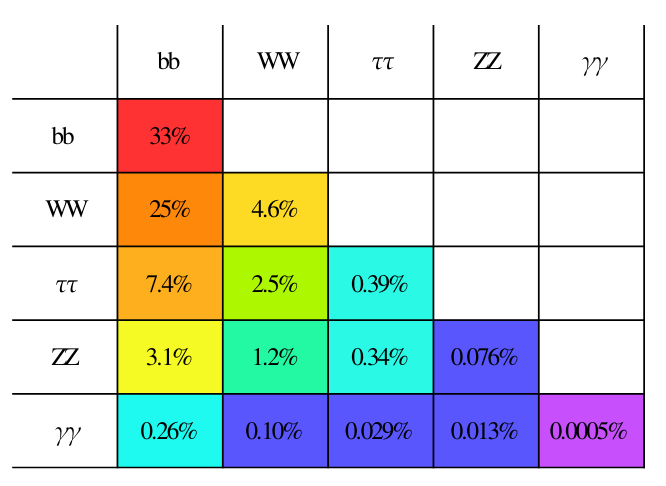
\includegraphics[width=0.5\textwidth]{Ch1/Img/HH_decays.png}
    \caption{Di-Higgs system decay branching ratios assuming SM Higgs bosons with $m_H=125.09$ GeV.}
    \label{fig:chap1:HH:HPD:DCY}
\end{figure}
Even other channels has a huge decay rate, $b\bar{b}\gamma\gamma$ final state is one of the most promising decay channels for the search for di-Higgs production as it has a good compromise between the very large branching ratio from $H\rightarrow b\bar{b}$ decay and the small Higgs to diphoton branching ratio. The $\gamma\gamma b\bar{b}$ channel is appealing thanks to an excellent diphoton resolution leads on a clean di-photon signature gives a narrow peak at Higgs mass in the $m_{\gamma\gamma}$ invariant mass spectrum
on top of a smoothly falling background. These helps in separating the signal from the background processes. This thesis is preformed on $\gamma\gamma b\bar{b}$ final state.
\subsection{Di-Higgs as a probe of BSM physics}
\label{chap1:HH:BSM}
\textcolor{red}{How \kl cloud probe the existence of BSM effects} \\
The small cross section (Eq. \ref{eq:chap1:HH:XSEC:NNL0}) is challenging to measure. If SM expectations hold, the production of a Higgs boson pair in a single pp interaction should not be observable with the currently available LHC data set, unless its cross section is enhanced by an anomalous (new physics). Which makes HH production a promising process to probe new physics beyond the standard model (BSM). Beyond the Standard-Model (BSM) scenarios may enhance the Higgs boson pair production rate and would be indicating a new physics. Many of those BSM theories predict the existence of heavy particles that can decay into a pair of Higgs bosons. These could be identified as a resonance in the di-Higgs invariant mass spectrum. In addition to the resonant production, there can also be non-resonant enhancements to the Higgs boson pair cross section. Only the non-resonance search is considered in this thesis. These can either originate from loop corrections involving new particles, such a light colored scalars, or through non-SM couplings. Anomalous couplings of Higgs boson with the top-quark or triple Higgs self-coupling can either be extensions to the SM, such as contact interactions between two top quarks and two Higgs bosons, or be deviation from the SM values of the trilinear Higgs coupling. Considering possible modifications of them, the deviation is quantified by \kl $ = \frac{\lambda_{HHH}}{\lambda_{HHH}^{SM}}$ and \kt $= \frac{\lambda_{t}}{\lambda_{t}^{SM}}$, where $\lambda_{i}$ is the coupling i of the new physics and $\lambda_{i}^{SM}$ its SM value. \\
Given the \kt and \kl modifiers, the Higgs pair production cross section can be parameterised as :
\begin{equation}
  \sigma \approx k_{t}^{4}\left[|\square|^{2}+\frac{k_{\lambda}}{k_{t}}(\square\bigtriangleup+\bigtriangleup \square)+\left(\frac{k_{\lambda}}{k_{t}}\right)^{2}|\bigtriangleup|^{2}\right], 
\end{equation}
this shows that the production cross section depends on both parameters \kt and \kl, while the kinematics only depends on their ratio, that modifies the relative contribution of the two diagrams and thus the shape of the kinematic distributions. The maximum interference between the two diagrams corresponds to the cross section minimum located at \kl = 2.4\kt. Figure \ref{fig:chap1:HH:BSM:I} shows an illustration of diagram contribution to the invariant mass distribution of di-Higgs system $m_{HH}$. The box diagram has an invariant mass spectrum peaking around 2$m_t$. When including the triangle diagram with the triple Higgs self-coupling, the invariant mass spectrum becomes generally softer with the increase of its contribution. This effect cause a large change in $m_{HH}$ distribution as shown in Figure \ref{fig:chap1:HH:BSM:MHH}.
\begin{figure}[H]
    \centering
    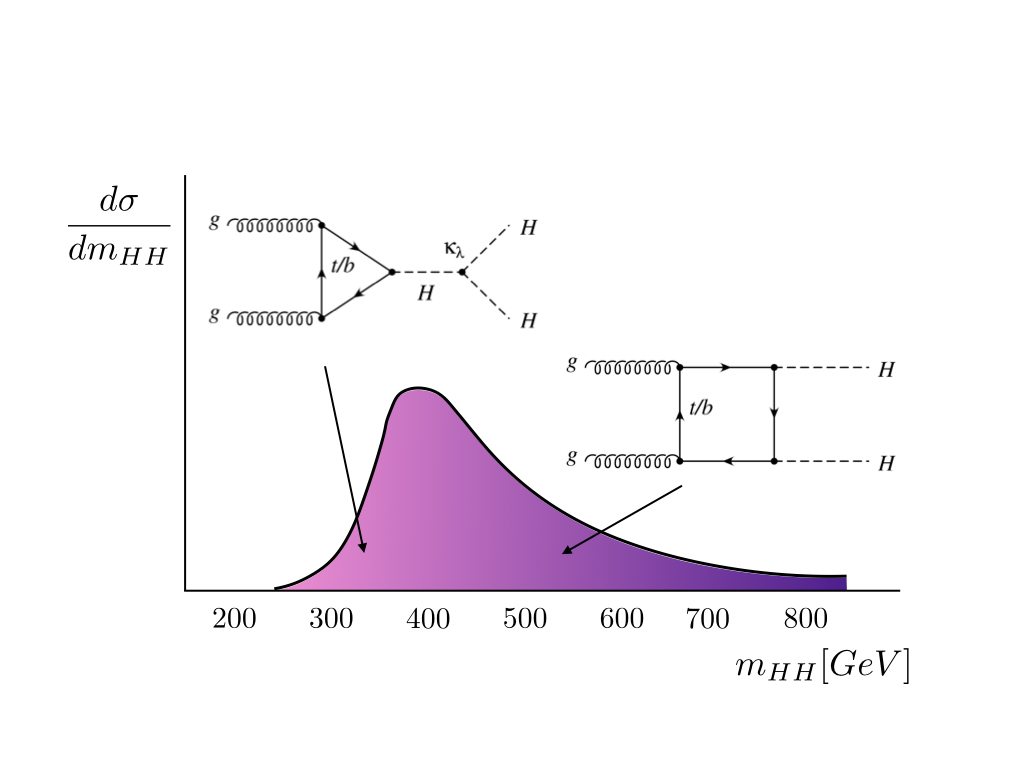
\includegraphics[width=0.5\textwidth]{Ch1/Img/illustration_mHH.jpeg}
    \caption{Illustration of both box and triangle diagrams contribution to di-Higgs invariant mass spectrum.}
    \label{fig:chap1:HH:BSM:I}
\end{figure}
The interference of the two diagrams also generates local minima in the differential cross section around $m_{HH}=2m_t$ for the case of \kl=2.
\begin{figure}[H]
    \centering
    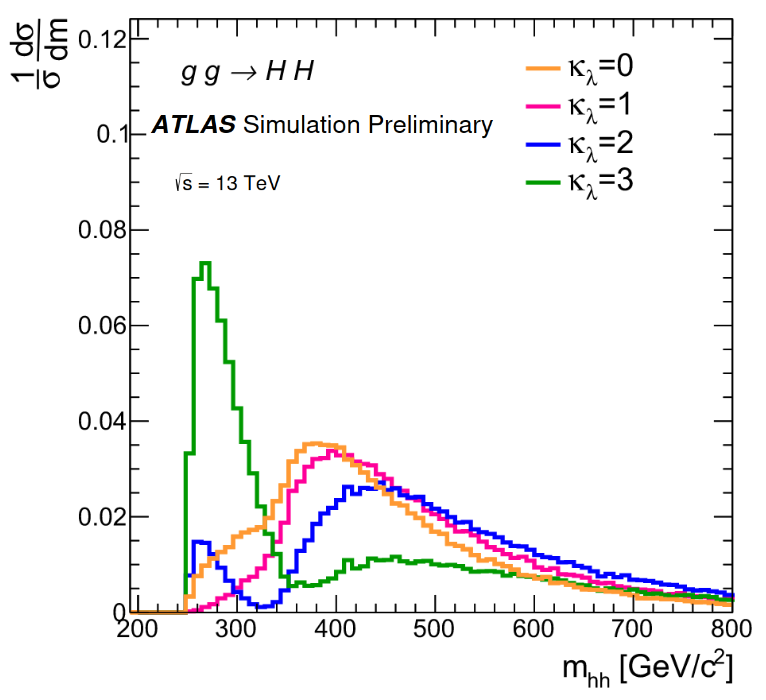
\includegraphics[width=0.5\textwidth]{Ch1/Img/mHH.png}
    \caption{Higgs pair invariant-mass distribution in ggF for various values of \kl assuming \kt=1.}
    \label{fig:chap1:HH:BSM:MHH}
\end{figure}

Figure \ref{fig:chap1:HH:BSM:XSEC:L} displays total LO and NLO cross sections for the six dominant HH production channels at the LHC with $\sqrt{s}=14$ TeV, as a function of the self-interaction coupling \kl. The SM value of the cross section corresponds to \kl=1. The corresponding cross section as a function of centre-of-mass energy is shown Figure \ref{fig:chap1:HH:BSM:XSEC:S}. As mentioned above, Higgs pair production is a promising process to probe new BSM physics. In this thesis, in addition to searching for the SM Higgs pair production process, constrain on \kl is also extracted.
\begin{figure}[H]
    \centering
    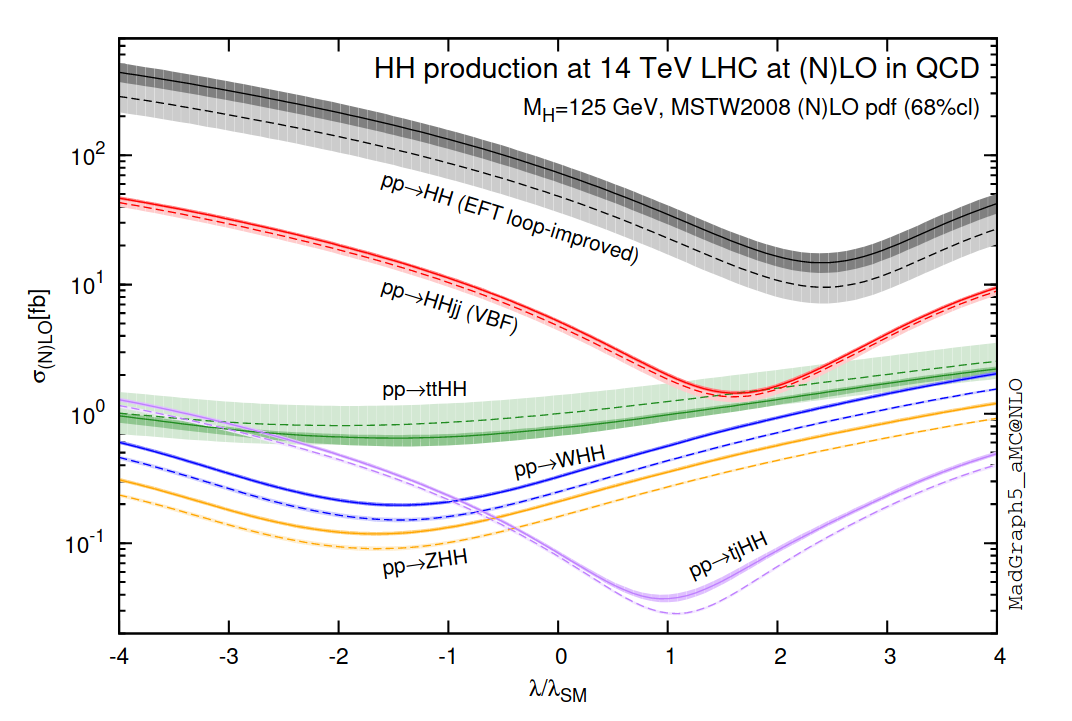
\includegraphics[width=0.5\textwidth]{Ch1/Img/HH_Xsec_as_lambda.png}
    \caption{Total LO and NLO cross sections for HH production at the LHC with $\sqrt{s}=14$ TeV, as a function of the self-interaction coupling \kl.}
    \label{fig:chap1:HH:BSM:XSEC:L}
\end{figure}
\begin{figure}[H]
    \centering
    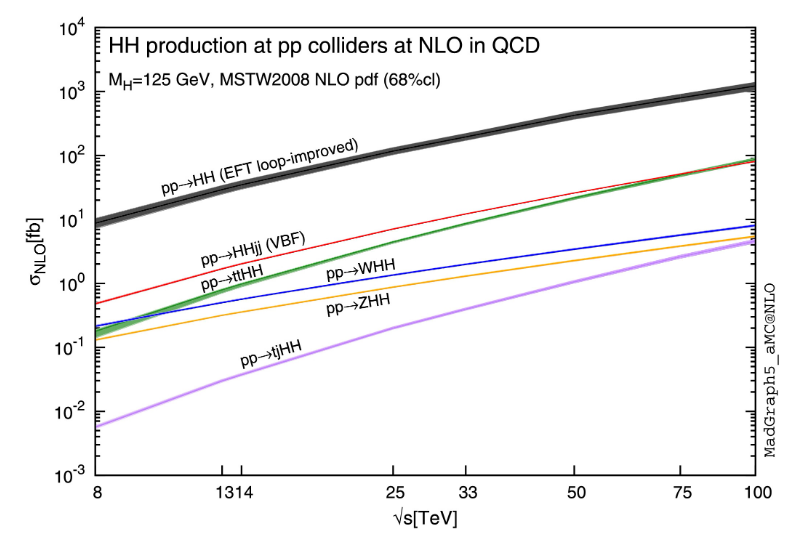
\includegraphics[width=0.5\textwidth]{Ch1/Img/HH_XSec_as_S.png}
    \caption{Total cross sections at the NLO for HH production as a function of centre-of-mass energy. Assuming \kl and \kt equals to their SM values.}
    \label{fig:chap1:HH:BSM:XSEC:S}
\end{figure}
\subsection{Current Measurements}
\label{chap1:HH:CM}
\textcolor{red}{This includes the 36 \ifb results and the limit on HH cross section and \kl.} \\
At the beginning of this thesis (2018), the latest measurement of Higgs pair production was preformed with an amount of data of 36.1\ifb representing the data collected by ATLAS detector in 2015 and 2016 (Chapter \ref{LHC&ATLAS} is dedicated to ATLAS detector). Results of the previous analysis were consistent with the SM expectations. In the non-resonant case, results are interpreted in the context of \kl. The analysis set an observed (expected) 95\% CL upper limit on HH cross section of 0.73 (0.93) pb, corresponding to 22 (28) times the predicted SM value. The Higgs self coupling is constrained to be between -8.2 $<$ \kl $<$ 13.2 at 95\% CL (-8.3$<$\kl$<$13.2 expected), other SM parameters are fixed to their expected value when extracting limits. The limit scan of \kl is shown in Figure \ref{fig:chap1:HH:CM:KL}. \\
Contributing to the \HHyybb non-resonant analysis involves 139\ifb of data collected during the Run 2 (2015-2018) of the LHC program, and improve the current limits on the cross-section and self-coupling is the aim of this thesis. 
\begin{table}[H]
    \centering
    \begin{tabular}{ccccc}
    \hline
         & Observed & Expected & -1$\sigma$ & +1$\sigma$ \\
    \hline
        $\sigma_{gg\rightarrow HH}$ [pb] & 0.73 & 0.93 & 0.66 & 1.3 \\
        As a multiple of $\sigma_{SM}$ & 22 & 28 & 20 & 40 \\
        \hline
    \end{tabular}
    \caption{The 95\% CL observed and expected limits on the Higgs boson pair cross-section in pb and as a multiple of the SM production cross-section. The $\pm1\sigma$ band around each 95\% CL limit is also indicated.}
    \label{tab:chap1:HH:CM:XSEC}
\end{table}
\begin{figure}[H]
    \centering
    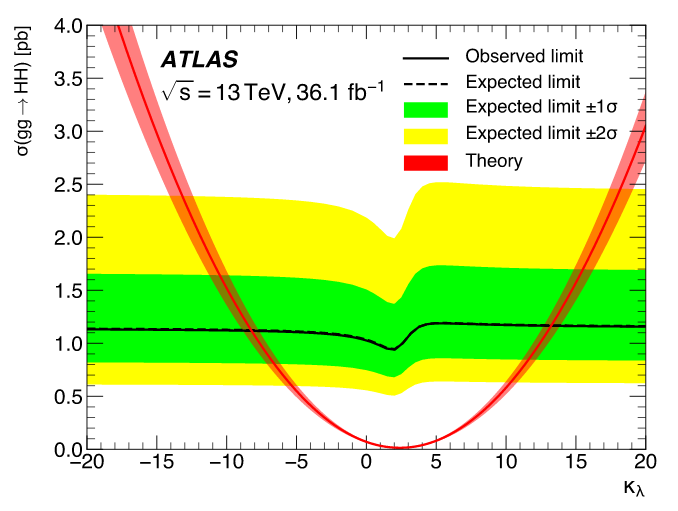
\includegraphics[width=0.5\textwidth]{Ch1/Img/kl_36ifb.png}
    \caption{The expected and observed 95\% CL limits on the non-resonant production cross section $\sigma_{gg\rightarrow HH}$ as a function of \kl. The red line indicates the predicted HH cross section if \kl is varied but all other couplings remain at their SM values. The red band indicates the theoretical uncertainty of this prediction.}
    \label{fig:chap1:HH:CM:KL}
\end{figure}
\section{Effective Field Theory (EFT)}
\label{chap1:EFT}
\textcolor{red}{A brief introduction to EFT and how it helps to probe physics at large scale.\\}
In the context of search for BSM physics, so far, no indication has been found at the LHC. This could be explained by the fact that the new physics is not accessible at the LHC. Effective Field Theories (EFTs) provide an approach to probe the existence of BSM physics in a model independent way at the LHC, even if the new physics scale $\Lambda$ is not directly accessible at the LHC. When BSM resides at scales larger than the EW scale ($\Lambda >> vev$), the new physics decouples from the SM and no light hidden states are produced. When this condition is satisfied, an expansion of the Lagrangian is canonical dimensions of $\frac{vev}{\lambda}$ can be performed. The theory that results is the Standard Model Effective Field Theory (SMEFT). The SMEFT is well defined and has been studied with increased theoretical sophistication in recent years, and it can capture a wide range of possible extensions of the SM. Such SM extensions can address the strong evidence for dark matter and neutrino masses not covered by SM. A linear EFT model of SMEFT is considered in this thesis : 
\begin{equation}
    \mathcal{L}_{S M E F T}=\mathcal{L}_{S M}+\mathcal{L}^{5}+\mathcal{L}^{6}+\mathcal{L}^{7}+\ldots, \quad \mathcal{L}^{d}=\sum_{i=1}^{n_{d}} \frac{C_{i}^{d}}{\Lambda^{d-4}} Q_{i}^{d} \quad for \ d>4.
\end{equation}
The number of non-redundant operators in $\mathcal{L}^i$ is known. The operators $Q_i^d$ are suppressed by d-4 powers of the cutoff scale $\Lambda$. These operators build a complete set of all operators allowed by the SM gauge symmetries. The Warsaw basis is used for the invariant operators $Q_i^d$. The coefficients $C_i^d$ are called Wilson coefficients. They are free parameters of the theory. \\
The new physics interferes with the standard model, and modify the kinematics of the given process. The cross section of a specific process within the SMEEFT can be splitted as : 
\begin{equation}
    \sigma = \sigma_{SM} + \sigma_{int} + \sigma_{BSM},
\end{equation}
where $\sigma_{SM}$ is the SM cross section, $\sigma_{int}$ represents the interference between the BSM physics with the SM, and $\sigma_{BSM}$ is a pure BSM physics suppressed by $\Lambda^{-4}$ that does not depend on the SM amplitude; it can however become important in specific regions of the phase space and its consideration can prevent negative cross sections. \\

Similarly to \kl variations, new physics can affect Higgs pair production. Higgs pair production results can benefit from an interpretation beyond the \kl variations. The full Run 2 di-Higgs results can be used to set limits on SMEFT parameters. Detailed studies of EFT within double Higgs context are described in the dedicated Chapter \textbf{To Be Added}.
\section{Conclusion}
\label{chap1:Conc}

\textcolor{red}{Brief conclusion of chapter 1.\\}
Higgs mechanism was introduced into the SM to explain the origin of the masses of the particles. A particle with similar proprieties to SM Higgs boson was discovered at collisions of LHC in 2012. After its discovery, a priority of the ATLAS and CMS collaborations has been to better understand its properties and couplings. Understanding Higgs self-coupling is vital providing a direct probe on electroweak symmetry breaking (EWSB) and reconstruct the Higgs potential to check whether the boson discovered is Higgs boson. The theoretical backgrounds needed to understand the main subject of the thesis are introduced. As well as the current results with 2015-2016 data. The EFT is highlighted as an interpretation of di-Higgs results beyond \kl. Next chapter focus on the experimental setup to produce and collect data, the Large Hadron Collider and the ATLAS detector. 

